In den nachfolgenden Unterkapitel werden die theoretischen Grundlagen erarbeitet, welche für das Verständnis sowie das
Design eines Demonstrators für das \acrshort{tof}-Verfahren notwendig sind.

\subsection{Time of Flight}

Beim Messverfahren, welches als \dq \acrlong{tof}\dq\ bekannt ist, geht es darum, die Laufzeit eines Signales zu messen.
Das Signal kann hierbei optischer oder akustischer Natur sein. Eine Anwendung davon ist beispielsweise die Distanzmessung.

Beim hier behandelten optischen Prinzip wird mit einem Sender Licht ausgesandt, welches von einem Empfänger detektiert wird.
Zwischen dem Senden und Empfangen des Signals kann eine Zeitmessung gemacht werden. Weil sich Licht mit einer definierten
Geschwindigkeit ausbreitet, kann über diese Laufzeitmessung ein Rückschluss darüber gewonnen werden, welche Distanz
das Signal innerhalb der gemessenen Zeit zurückgelegt hat.

\begin{figure}[H]
    \centering
    \includegraphics[width=\textwidth]{diagrams/dToF_vs_iToF.pdf}
    \caption{Visualisierung von a: direct \acrshort{tof} und b: indirect \acrshort{tof}}\label{fig:dtof_vs_itof}
\end{figure}

Man unterscheidet zwei Arten von \acrshort{tof}: Direct \acrshort{tof} (dToF) und Indirect \acrshort{tof} (iToF). Bei dToF
wird einzig und alleine die Laufzeit zwischen Sende- und Empfangspuls ermittelt. In der Abbildung~\ref{fig:dtof_vs_itof}
sind bei a) beispielhaft solche Pulse dargestellt.

Bei iToF wird (teilweise zusätzlich) zur Laufzeitmessung auch die Phasenverschiebung eines modulierten Lichtsignales gemessen.
Dies sei bei Abbildung~\ref{fig:dtof_vs_itof} im Teil b) dargestellt. Diese Methode erlaubt es, höhere Auflösungen zu
erreichen, ist jedoch in der Auswertung und Signalaufbereitung ungleich komplexer.

Diese Arbeit beschränkt sich auf das direct \acrshort{tof} Verfahren.

Nachfolgend werden die theoretischen Grundlagen, vor allem in Hinblick auf das Auslegen einer geeigneten Optik, diskutiert.

\pagebreak

\subsection{Photostrom}

Zur Berechnung des theoretisch zu erwartenden Photostroms wird von einer Distanz von $10~m$ zur Wand ausgegangen.

In einer vereinfachten Betrachtung treffe ein Laserstrahl mit einer Divergenz von $0\degree$ rechtwinklig auf eine Wand
und werde dort uniform Halbkugel-förmig gestreut. In der Realität wird der Laser nicht mit $0\degree$ zur Wand gehen und
die Streuung wird sich nicht uniform verteilen, sondern in der Mitte stärker konzentriert sein.

Die Berechnung der empfangenen Strahlungsleistung, der Strahlungsintensität, dem Raumwinkel einer Halbkugel und dem
Photostrom sind in Formel~\ref{eq:pin}, \ref{eq:ie}, \ref{eq:omega} bzw. \ref{eq:iph} gezeigt.

\begin{equation}\label{eq:pin}
    P_{in} = E_e \cdot A = \frac{I_e}{r^2} \cdot A
\end{equation}
\myequations{Eintreffende Lichtleistung}

\begin{equation}\label{eq:ie}
    I_e = \frac{P_{out}}{\Omega}
\end{equation}
\myequations{Strahlungsintensität}

\begin{equation}\label{eq:omega}
    \Omega = 4\cdot \pi \cdot 0.5
\end{equation}
\myequations{Raumwinkel}

\begin{equation}\label{eq:iph}
    I_{ph} = S \cdot P_{in}
\end{equation}
\myequations{Photostrom}

\subsubsection{Berechnung mit RLD94PZJ5 und BPV23NF}

Erste Berechnungen werden mit der Laserdiode RLD94PZJ5 \cite{rohm2020rld94pzj5_datasheet} und der Photodiode BPV23NF
\cite{vishay2024bpv23nf_datasheet} durchgeführt.

Die relevanten Werte aus den Datenblättern sind in Formel~\ref{eq:rld94pzj5_num} und \ref{eq:rbpv23nf_num} aufgelistet.

\begin{equation}\label{eq:rld94pzj5_num}
    P_{out} = 285~mW
\end{equation}
\myequations{Werte des RLD94PZJ5}

\begin{equation}\label{eq:rbpv23nf_num}
    \begin{split}
        A &= 4.4~mm^2\\
        S &= 0.6~\frac{A}{W}
    \end{split}
\end{equation}
\myequations{Werte des BPV23NF}

Diese Werte eingesetzt in Formel~\ref{eq:ie}, \ref{eq:pin} und \ref{eq:iph} ergibt die Resultate in
Formel~\ref{eq:rld94pzj5_rbpv23nf_num}.

\begin{equation}\label{eq:rld94pzj5_rbpv23nf_num}
    \begin{split}
        I_e    &= \frac{P_{out}}{\Omega} = \frac{285~mW}{4\cdot \pi \cdot 0.5~sr} = 45.4~\frac{mW}{sr}\\
        P_{in} &= \frac{I_e}{r^2} \cdot A = \frac{45.4~\frac{mW}{sr}}{(10~m)^2} \cdot 4.4~mm^2 = 2~nW\\
        I_{ph} &= S \cdot P_{in} = 0.6~\frac{A}{W} \cdot 2~nW = 1.2~nA
    \end{split}
\end{equation}
\myequations{Nummerische Resultate mit RLD94PZJ5 und BPV23NF}

\subsubsection{Berechnung mit RLD65NZX1 and NJL6401R-3}

Die Laserdiode RLD94PZJ5 hat im Bezug auf diese Projektarbeit zwei Nachteile: Einerseits besitzt sie eine so hohe Leistung,
dass sie für das menschliche Auge schädigend wirken kann. Andererseits strahlt sie in einem Wellenlängenbereich ab, der
für das menschliche Auge nicht sichtbar ist.

Aus diesen Gründen wird eine zweite Laserdiode evaluiert: RLD65NZX1 \cite{rohm2019rld65nzx1_datasheet}. Gepaart wird
sie mit der Photodiode NJL6401R-3 \cite{jrc2014njl6401r3_datasheet}. Die folgenden Berechnungen werden basierend auf
diesen beiden Komponenten durchgeführt.

Die relevanten Werte aus den Datenblättern sind in Formel~\ref{eq:rld65nzx1_num} und \ref{eq:njl6401r3_num} aufgelistet.

\begin{equation}\label{eq:rld65nzx1_num}
    P_{out} = 10~mW
\end{equation}
\myequations{Werte des RLD65NZX1}

\begin{equation}\label{eq:njl6401r3_num}
    \begin{split}
        A &= 0.7~mm \cdot 0.7~mm = 0.49~mm^2\\
        S &= 0.42~\frac{A}{W}
    \end{split}
\end{equation}
\myequations{Werte des NJL6401R-3}

Eingesetzt in die Formeln~\ref{eq:ie}, \ref{eq:pin} und \ref{eq:iph} ergeben sich die neuen Resultate in
Formel~\ref{eq:rld65nzx1_njl6401r3_num}.

\begin{equation}\label{eq:rld65nzx1_njl6401r3_num}
    \begin{split}
        I_e    &= \frac{P_{out}}{\Omega} = \frac{10~mW}{4\cdot \pi \cdot 0.5~sr} = 1.59~\frac{mW}{sr}\\
        P_{in} &= \frac{I_e}{r^2} \cdot A = \frac{1.59~\frac{mW}{sr}}{(10~m)^2} \cdot 0.49~mm^2 = 7.8~pW\\
        I_{ph} &= S \cdot P_{in} = 0.42~\frac{A}{W} \cdot 7.8~pW = 3.28~pA
    \end{split}
\end{equation}
\myequations{Nummerische Resultate mit RLD65NZX1 and NJL6401R-3}

\subsubsection{Berechnung mit Empfangs-Linse}

Auf Vorschlag der Dozenten werden verschiedene Optiken aus einem Baukasten-System von QIOPTIQ ausprobiert.
Besonders vielversprechend erscheint hierbei eine Linse mit einem Durchmesser von 17~mm bei einer Brennweite von
40~mm. Die Linse ist in Abbildung~\ref{fig:lens} dargestellt.

\begin{figure}[H]
    \centering
    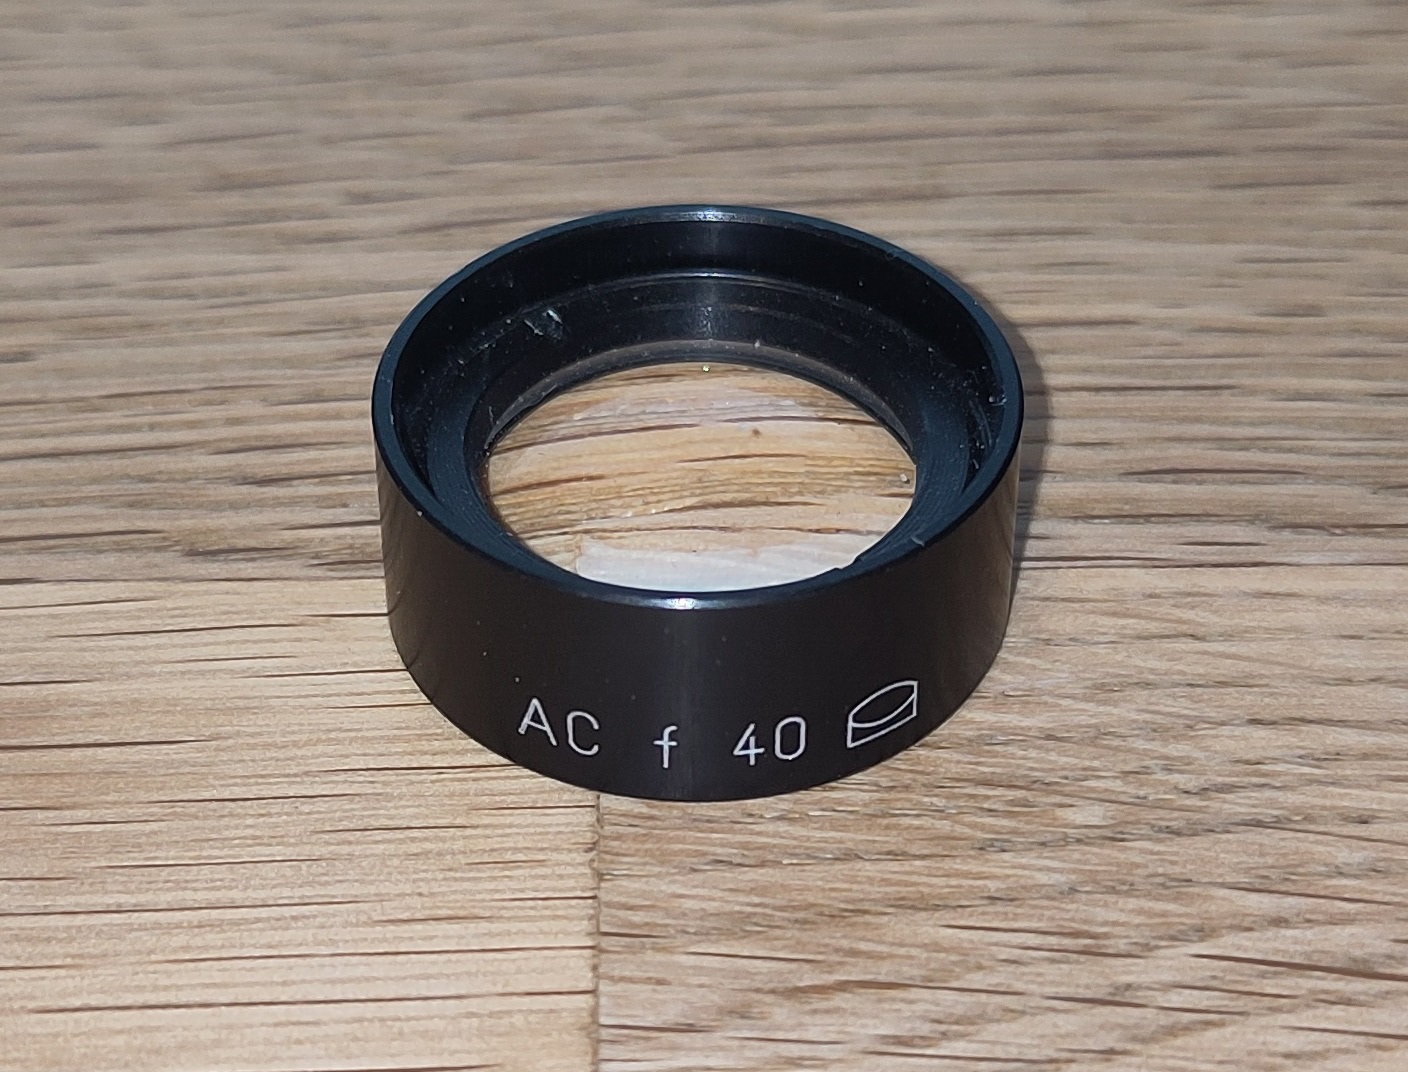
\includegraphics[width=0.5\textwidth]{graphics/photo_lens.jpg}
    \caption{Linse von QIOPTIQ}\label{fig:lens}
\end{figure}

Eine solche Linse vergrössert die effektive Fläche, auf welcher der Lichtstrom empfangen werden kann. Dies hat
eine höhere Empfangsleistung, sprich einen höheren Lichtstrom, zur Folge.

Die Formel~\ref{eq:njl6401r3_lens} zeigt die beim Einsatz einer solchen Optik zu erwartende Flächenvergrösserung.

\begin{equation}\label{eq:njl6401r3_lens}
    A' = \frac{A_{L}}{A_{PD}} = \frac{(\frac{17~mm}{2})^2 \cdot \pi}{0.49~mm^2} = 463.2
\end{equation}
\myequations{Vergrösserung der Empfangsfläche durch Linse}

\subsubsection{Erwarteter Lichtstrom}
Nachfolgend werden zwei Szenarien betrachtet: Einmal wird wie bis anhin davon ausgegangen, dass sich das Licht ab dem Laser
in einem gebündelten Strahl ausbreitet, um danach halbkugelförmig und diffus am Target zu reflektieren.

Im zweiten Szenario wird versucht, die Abstrahlcharakteristik der Laser-Diode zu modellieren. Laut Datenblatt hat die
Diode in der Abstrahlebene zwei unterschiedliche Öffnungswinkel, was mit dem Raumwinkel einer rechteckigen Pyramide
annäherungsweise berechnet werden kann. Die Streuung wird verhindert, da an einem Spiegel reflektiert wird.

Bei beiden Szenarien sei die abgestrahlte Leistung der Laser-Diode höher als in der ersten Rechnung. Im gepulsten
Betrieb kann diese problemlos über das maximale Rating erhöht werden. Thermisch stellt dies kein Problem für die Diode dar, da
der Duty-Cycle sehr klein ist. Die Formel~\ref{eq:rld65nzx1_higher_output} zeigt die neu zu erwartete Abstrahl-Leistung
eines solchen Pulses. Die Effizienz der Laser-Diode wird dem Datenblatt des RLD65NZX1 entnommen \cite{rohm2019rld65nzx1_datasheet}.

\begin{equation}\label{eq:rld65nzx1_higher_output}
    \begin{split}
        \eta     &= \frac{P_{25~mA}}{I_{ld}} = \frac{7~mW}{25~mA} = 0.28~\frac{W}{A}\\
        I_{ld}'  &= \frac{5~V - V_{LD}}{R_{v}} = \frac{5~V - 2.8~V}{5~\Omega} = 440~mA\\
        P_{out}' &= \eta \cdot I_{ld}' = 0.28~\frac{W}{A} \cdot 440~mA = 123~mW
    \end{split}
\end{equation}
\myequations{Erhöhte Sendeleistung bei der Laser-Diode}

Bei einem Target, welches sich in 2~m Distanz befindet, kann nach Formel~\ref{eq:photocurrent_scenario1} folgender
Lichtstrom erwartet werden:

\begin{equation}\label{eq:photocurrent_scenario1}
    \begin{split}
        P_{in} &= \frac{P_{out}}{\Omega \cdot r^2} \cdot A_{L} = \frac{123~mW}{4\pi \cdot 0.5~sr \cdot (2~m)^2} \cdot 227~mm^2 = 1.11~\mu W\\
        I_{ph} &= S \cdot P_{in} = 0.42~\frac{A}{W} \cdot 1.11~\mu W = 467~nA
    \end{split}
\end{equation}
\myequations{Photostrom Szenario 1}

Ohne Optik strahlt die Laserdiode keinen gebündelten Strahl. Diese Abstrahlcharakteristik sei im zweiten Szenario über
den Raumwinkel einer Pyramide, wie er in Formel~\ref{eq:solid_angle_pyramid} definiert ist, modelliert. Die typischen
Abstrahlwinkel $\theta$ werden ebenfalls dem Datenblatt der Laser-Diode entnommen. Hierbei ist zu beachten, dass im
Datenblatt der Vollwinkel angegeben wird. Der Wert in der Formel wird deswegen halbiert.

\begin{equation}\label{eq:solid_angle_pyramid}
    \Omega_{P} = 4 \cdot arcsin(sin(\theta_x) \cdot sin(\theta_y)) =  4 \cdot arcsin \parenth*{sin \parenth*{\frac{9\degree}{2}} \cdot sin \parenth*{\frac{29\degree}{2}}} = 4.2~sr
\end{equation}
\myequations{Modell Abstrahlung Laserdiode}

Mit der Formel~\ref{eq:photocurrent_scenario2} wird erneut die zu erwartende Empfangsleistung sowie der dazugehörige
Photostrom berechnet. Der Unterschied zur vorherigen Berechnung liegt nun aber darin, dass der Raumwinkel auch bereits
vor der Reflexion berücksichtigt werden muss. Deswegen wird die Distanz zum Target mit zwei multipliziert.

\begin{equation}\label{eq:photocurrent_scenario2}
    \begin{split}
        P_{in} &= \frac{P_{out}}{\Omega \cdot (2 \cdot r)^2} \cdot A_{L} = \frac{123~mW}{4.2~sr \cdot (2 \cdot 2~m)^2} \cdot 227~mm^2 = 416~nW\\
        I_{ph} &= S \cdot P_{in} = 0.42~\frac{A}{W} \cdot 416~nW = 175~nA
    \end{split}
\end{equation}
\myequations{Photostrom Szenario 2}

\pagebreak

\subsection{Transimpedanzverstärker}

Wie die Berechnungen in den vorgängigen Kapiteln aufzeigen, besitzen die Photoströme, welche zu detektieren sind, sehr kleine
Stromstärken. Weiter sind die Lichtimpulse typischerweise oft nur von sehr kurzer Dauer, nämlich im Bereich einiger Nanosekunden.
Dies hat zur Folge, dass die Signale dementsprechend kurze Anstiegszeiten haben, welche es zu detektierten gilt.

Die Anforderungen deuten darauf hin, dass ein Verstärker mit sehr hohem Gain bei gleichzeitig sehr hoher Bandbreite eingesetzt werden muss.
Die Verstärkerschaltung, welche eingesetzt wird, ist ein Strom-Spannungswandler. Eine solche Beschaltung des Operationsverstärkers,
wie sie in Abbildung~\ref{fig:theory_tia} zu sehen ist, wird auch Transimpedanzverstärker (\acrshort{tia}) genannt.

\begin{figure}[H]
    \centering
    \includegraphics[width=0.5\textwidth]{diagrams/tia.pdf}
    \caption{Beschaltung Operationsverstärker als \acrshort{tia}}\label{fig:theory_tia}
\end{figure}

Wie der Name der Schaltung vermuten lässt, wandelt der Transimpedanzwandler den Photostrom \lstinline|Id| in eine Spannung
\lstinline|Vout| um. Dabei gibt der Feedback-Widerstand \lstinline|Rf| die Verstärkung vor, wie die Formel~\ref{eq:tia_simple}
zeigt:

\begin{equation}\label{eq:tia_simple}
    V_{out} = -R_{f} \cdot I_{d}
\end{equation}
\myequations{Übertragungsfunktion \acrshort{tia}}
